\documentclass[12pt,a4paper]{article}
\usepackage{pgf}
% \usepackage[condensed,math]{kurier}
% \usepackage[T1]{fontenc}
\usepackage{svg}
\usepackage{tikz}
\usepackage{stanli}
\usepackage{afterpage}
\usepackage{multirow}
\usepackage{subfig}
\usepackage{pgfpages}
\usepackage{rotating}

%\usepackage{times}


\pgfpagesdeclarelayout{boxed}
{
	\edef\pgfpageoptionborder{0pt}
}
{
	\pgfpagesphysicalpageoptions
	{%
		logical pages=1,%
	}
	\pgfpageslogicalpageoptions{1}
	{
		border code=\pgfsetlinewidth{2pt}\pgfstroke,%
		border shrink=\pgfpageoptionborder,%
		resized width=.9\pgfphysicalwidth,%
		resized height=.9\pgfphysicalheight,%
		center=\pgfpoint{.5\pgfphysicalwidth}{.5\pgfphysicalheight}%
	}%
}

\pgfpagesuselayout{boxed}


% Language setting
% Replace `english' with e.g. `spanish' to change the document language
\usepackage[english]{babel}

% Set page size and margins
% Replace `letterpaper' with `a4paper' for UK/EU standard size
\usepackage[a4paper,top=2cm,bottom=1.5cm,left=1.5cm,right=1.5cm,marginparwidth=1.75cm]{geometry}

% Useful packages
\usepackage{amsmath}
\usepackage{graphicx}
\usepackage[colorlinks=true, allcolors=blue]{hyperref}

\title{}
\author{}
\date{}

\begin{document}
	
	\newcommand{\subf}[2]{%
		{\small\begin{tabular}[t]{@{}c@{}}
				#1\\#2
		\end{tabular}}%
	}
	
	\begin{titlepage}
		\begin{center}
			
			\textbf{}
            
\includegraphics[width=1\textwidth]{utt.png}

            \vspace*{3cm}

			\vspace{1.5cm}
			
			\Huge
			\textbf{Zenith: Progressive Web Application}
            \textbf{Second project progress review}
			
			\vspace{0.8cm}
			\large
			
			\vspace{0.5cm}
			\LARGE
			
			
			\vfill
			
			
			
			\vspace{0.8cm}
			
			
			
			\Large
			
			
			
			
		\end{center}
		\Large
		\begin{tabbing}
			\hspace*{1em}\= \hspace*{8em} \= \kill % set the tabbings
            \> \>\textbf{García Gonzalez Christian Andrés} \\
            \> \> \textbf{López Bautista Cristian Alexis} \\
             \> \>  \textbf{Mercado Juárez Ángel Hayr} \\
             \> \>  \textbf{Salas Díaz Guillermo} \\
			\> Name:\>  \textbf{Santillán Galaviz Ken Antonio} \\
			\> Group:\>  10-B \\
			\> Subject:\>  Progressive Web Applications  \\
			\> Professor:  \> Dr. Ray Brunet Parra Galaviz \\
			\> Date: \>  Wednesday, February 6th, 2024
		\end{tabbing}
		
	\end{titlepage}
	
	\section{Backend Progress}
    
    \subsection{Database}

    \paragraph{As part of the progress of the project in the backend, we have created the entire database, from the design of diagrams to the creation and insertion of some test data using data generation libraries such as faker. This database is already hosted on an AWS server for remote access.}

    \begin{figure}[ht]
      \centering
      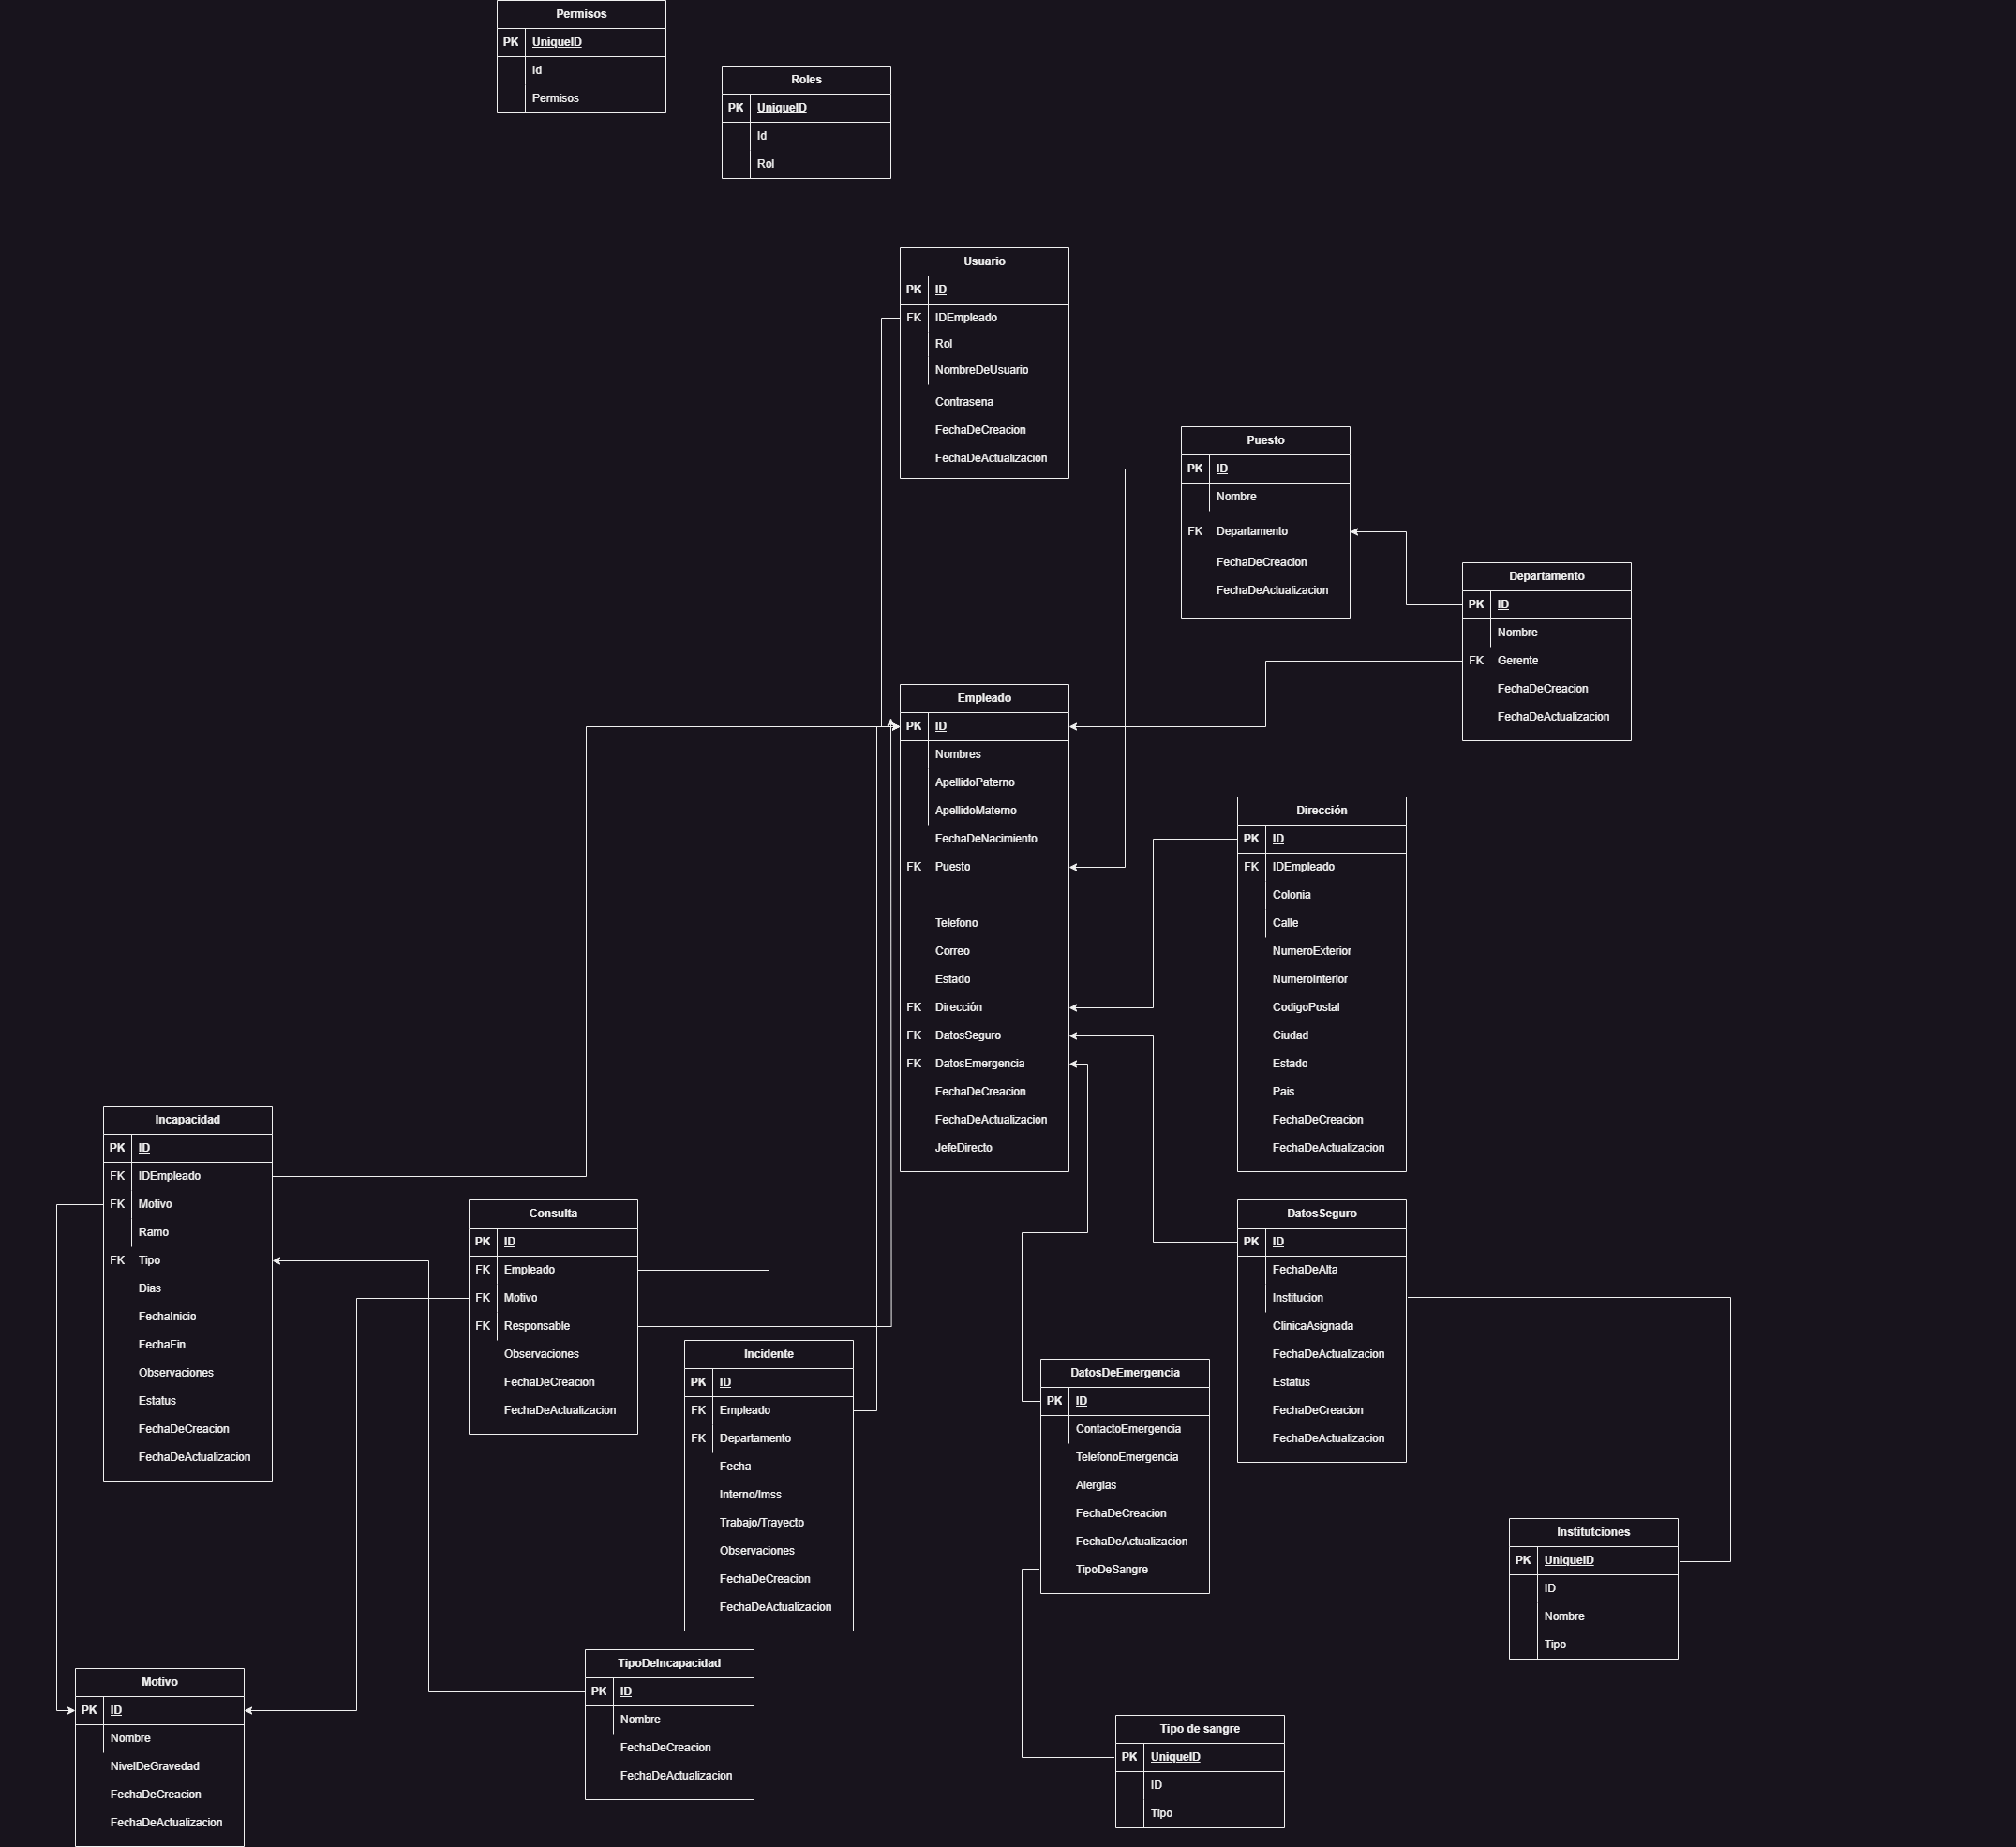
\includegraphics[width=0.5\textwidth]{diagram.png}
      \caption{Database diagram.}
    \end{figure}

    \begin{figure}[ht]
      \centering
      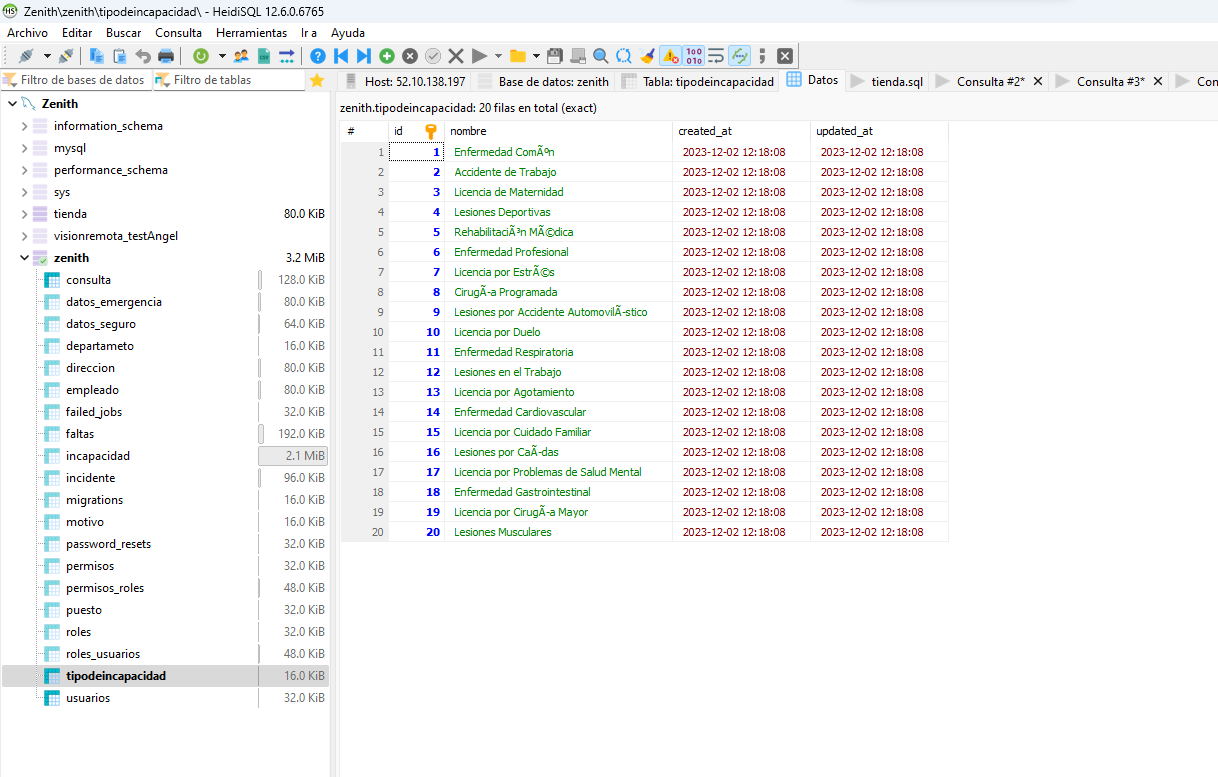
\includegraphics[width=0.5\textwidth]{database.png}
      \caption{Database.}
    \end{figure}

    \clearpage

    \subsection{API}

    \paragraph{The API created in Laravel is also located on the AWS server, consuming data from the database. This has all the necessary methods for the proper functioning of the app, as well as enough endpoints to have a good organization of data and requests.}

   \begin{figure}[ht]
      \centering
      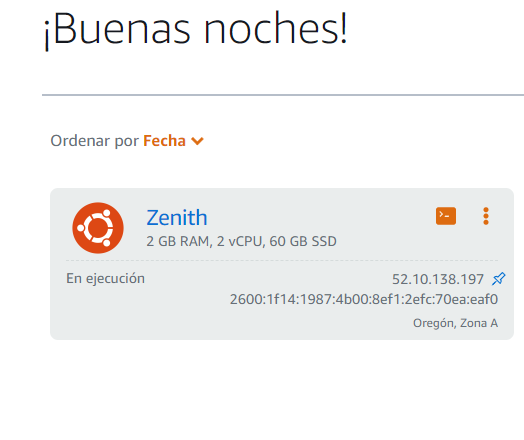
\includegraphics[width=0.5\textwidth]{server.png}
      \caption{Server in AWS.}
    \end{figure}

    \subsection{Requests}

    \paragraph{As a way to consume this API through requests when developing, the postman tool is used, in which we have created a team where the collection of requests that can be made to the API is located, as well as functional examples for testing.}

    \begin{figure}[ht]
      \centering
      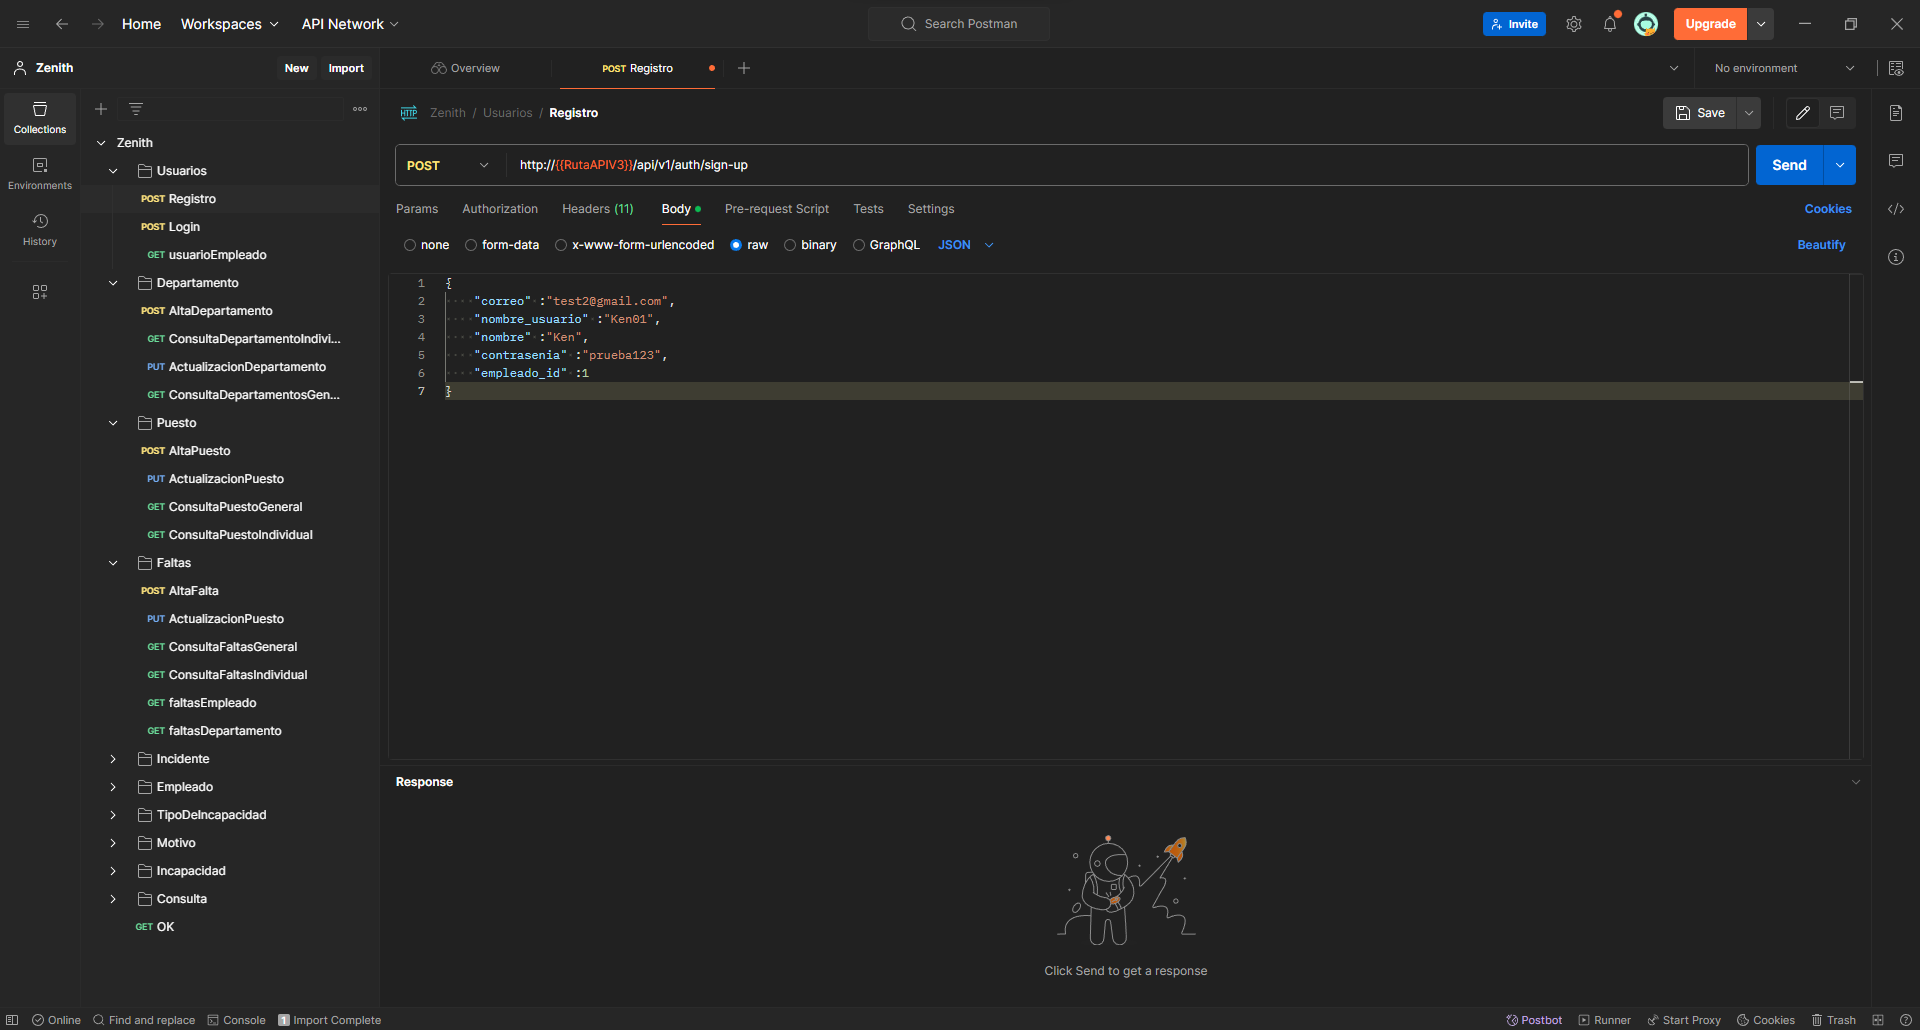
\includegraphics[width=0.5\textwidth]{postman.png}
      \caption{Postman collection.}
    \end{figure}

    \clearpage

    \section{Frontend Progress}
    
    \subsection{Mockups}

    \paragraph{In frontend development, we are using mockups created in the Proto.io tool, thanks to these we have some bases which we can follow to continue developing the views for the mobile application.}

    \begin{figure}[ht]
      \centering
      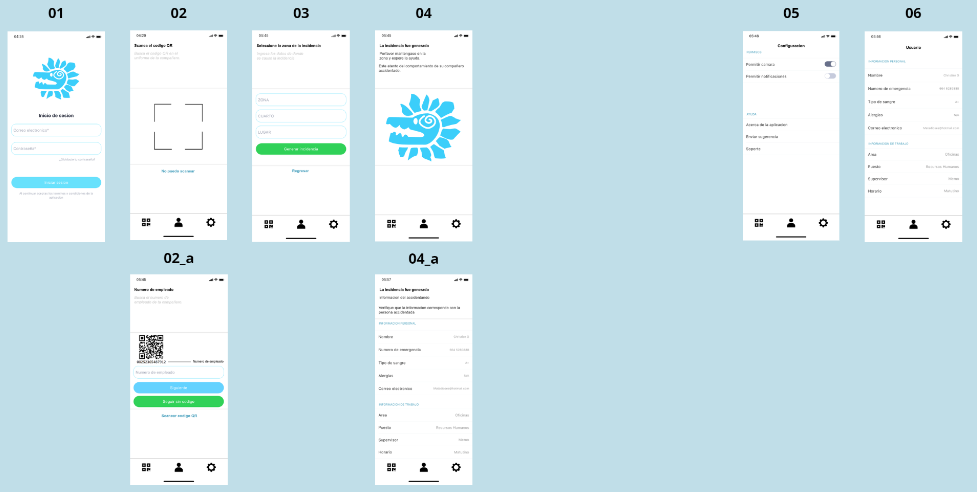
\includegraphics[width=0.5\textwidth]{mockups.png}
      \caption{Mockup compilation.}
    \end{figure}

    \subsection{PWA Design}

    \paragraph{On the PWA side, we are already creating the first views using react and based on the mockups shown above, we are also working on the generation and reading of QR codes, since this will be one of the main functions of our system.}

    \begin{figure}[ht]
      \centering
      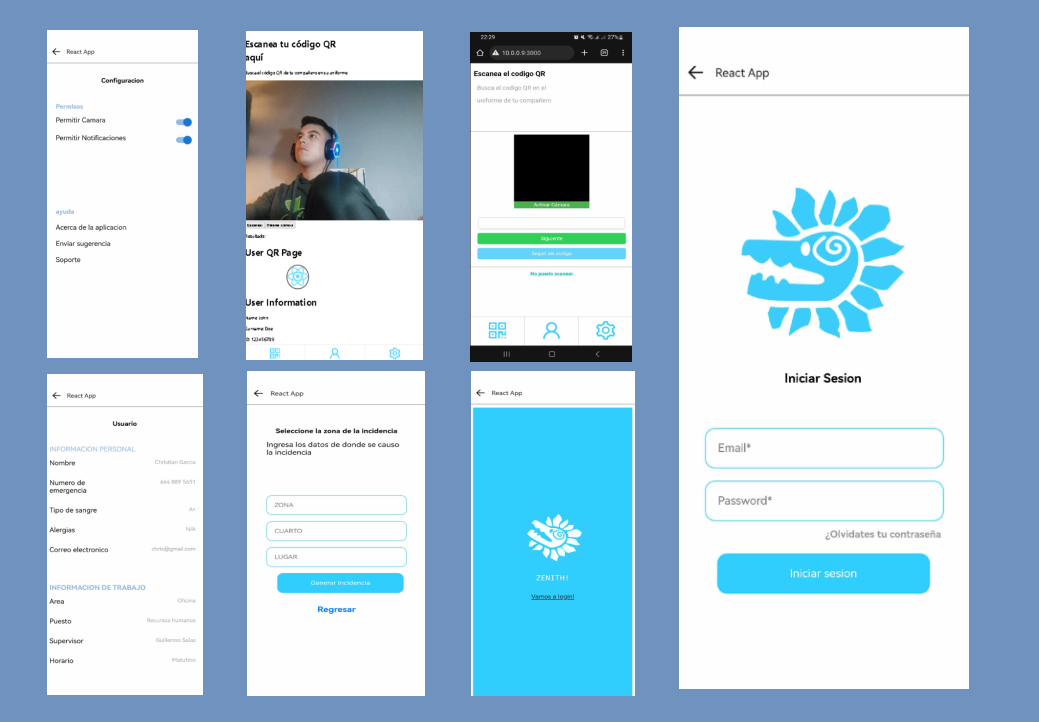
\includegraphics[width=0.5\textwidth]{pwa.png}
      \caption{PWA Screen compilation.}
    \end{figure}
	
\end{document}